%% LyX 2.1.0dev created this file.  For more info, see http://www.lyx.org/.
%% Do not edit unless you really know what you are doing.
\documentclass[english,conference]{IEEEtran}
\usepackage[T1]{fontenc}
\usepackage[utf8]{luainputenc}
\usepackage{array}
\usepackage{multirow}
\usepackage{amsmath}
\usepackage{amssymb}
\usepackage{stmaryrd}
\usepackage{graphicx}

\makeatletter

%%%%%%%%%%%%%%%%%%%%%%%%%%%%%% LyX specific LaTeX commands.
%% Because html converters don't know tabularnewline
\providecommand{\tabularnewline}{\\}

%%%%%%%%%%%%%%%%%%%%%%%%%%%%%% User specified LaTeX commands.


% manually specify the path to it: e.g.,
% \documentclass[conference]{../sty/IEEEtran}

\usepackage{times}\usepackage{psfig}% Add all your packages here

% correct bad hyphenation here
\hyphenation{op-tical net-works semi-conduc-tor IEEEtran}

\IEEEoverridecommandlockouts    % to create the author's affliation portion
                % using \thanks

\textwidth 178mm    % <------ These are the adjustments we made 10/18/2005
\textheight 239mm   % You may or may not need to adjust these numbers again
\oddsidemargin -7mm
\evensidemargin -7mm
\topmargin -6mm
\columnsep 5mm

\makeatother

\usepackage{babel}
\begin{document}
% paper title: Must keep \ \\ \LARGE\bf in it to leave enough margin.



\title{\ \\
 \textbf{A Fuzzy/Probabilistic Approach to Uncertain Interval Algebra}}


\author{Keyvan Mir Mohammad Sadeghi and Ben Goertzel}

\maketitle
% make the title area

\begin{abstract}
A novel approach to uncertain temporal inference is presented. Allen's
Interval Algebra is extended to fuzzy time-intervals via representing
the latter as trapeziums with distinct beginning, middle and end.
An uncertain version of the Interval Algebra composition table is
developed via running a computer simulation in which a large number
of fuzzy time-intervals are drawn from an assumed probability distribution,
and using machine learning to induce uncertain compositional rules
that hold approximately across the corpus of simulated intervals. 
\end{abstract}
% no key words



\section{Introduction}

\PARstart{B}{en} can write a couple intro paragraphs \cite{PLN}


\subsection{\label{sub:Allen-Interval-Algebra}Allen Interval Algebra}

One way to approach temporal reasoning is to represent the events
in terms of \emph{intervals}. An interval captures some portion of
time within which some features hold, then a temporal event could
be represented as \textbf{\emph{{[}a, b{]}}} where \emph{a} is the
beginning time-step of the event and \emph{b} is the ending. There
has been many works focused on addressing interval handling for temporal
inference, most notable of these are Allen's Interval Algebra (IA)
\cite{Allen} and Interval Temporal Logic (ITL) \cite{Moszkowski-Thesis,Moszkowski-Paper}. 

The foundation that IA is built on in treating intervals is to set
aside the actual time frames in which events occur, and instead, work
with the \emph{relation} between two intervals. To this end, IA defines
thirteen basic relations that address three desired qualities:
\begin{description}
\item [{Distinct}] the set of 13 relations constitute a partitioning over
the relation space
\item [{Exhaustive}] any pair of intervals can only be described by only
one of the relations
\item [{Qualitative}] the ground for comparing two intervals is how they
relate, as opposed to the time frames they lay in (quantitative)
\end{description}
Each Allen relation poses four constraints, for two intervals to be
qualified as holding the relation, they should satisfy all four. For
instance, assuming two intervals \emph{a} and \emph{b} are given,
the relation \emph{\{s\}} (starts) is defined as 1) $beginning_{a}=beginning_{b}$
2) $beginning_{a}<ending_{b}$ 3) $ending_{a}>beginning_{b}$ 4) $ending_{a}<ending_{b}$.
The set of thirteen Allen relations are shown in Table \ref{tab:Temporal-Relations}.

Having the relations in place, IA continues with defining operations
on relations:
\begin{description}
\item [{Complement}] denoted as \emph{\textasciitilde{}r}, complement of
set \emph{r} is the set of all relations not present in \emph{r}
\item [{Converse}] or \emph{!r}, is the set of relations obtained from
substituting intervals \emph{a} and \emph{b} in the original relation
\emph{a\{r\}b}
\item [{Intersection}] shown by \emph{r\textasciicircum{}s} is the set
of relations present in both \emph{r} and \emph{s}
\item [{Union}] \emph{r+s}, set of relations present in either \emph{r}
or \emph{s}
\item [{Composition}] \emph{r.s}, the set of all possible relations for
intervals \emph{a} and \emph{c} having \emph{a\{r\}b} and \emph{b\{s\}c}
\end{description}
Examples for these operations are presented in Table \ref{tab:Examples-of-operations}
and Table \ref{tab:Composition} shows composition of \emph{a\{r\}b}
and \emph{b\{s\}c} for singular \emph{r} and \emph{s}.

\begin{table}
\begin{centering}
\begin{tabular}{|c|c|c|}
\hline 
Precedes \emph{(p)} & Meets \emph{(m)} & Overlaps \emph{(o)}\tabularnewline
\hline 
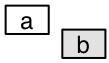
\includegraphics[scale=0.4]{p} & 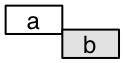
\includegraphics[scale=0.4]{m} & 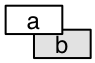
\includegraphics[scale=0.4]{o}\tabularnewline
\hline 
Preceded by \emph{(P)} & Met by \emph{(M)} & Overlapped by \emph{(O)}\tabularnewline
\hline 
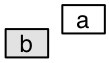
\includegraphics[scale=0.4]{pi} & 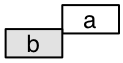
\includegraphics[scale=0.4]{mi} & 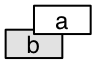
\includegraphics[scale=0.4]{oi}\tabularnewline
\hline 
Finished by \emph{(F)} & Contains \emph{(D)} & Starts \emph{(s)}\tabularnewline
\hline 
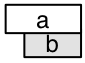
\includegraphics[scale=0.4]{fi} & 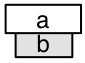
\includegraphics[scale=0.4]{di} & 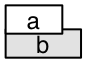
\includegraphics[scale=0.4]{s}\tabularnewline
\hline 
Finishes \emph{(f)} & During \emph{(d)} & Started by \emph{(S)}\tabularnewline
\hline 
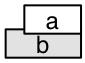
\includegraphics[scale=0.4]{f} & 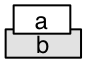
\includegraphics[scale=0.4]{d} & 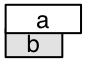
\includegraphics[scale=0.4]{si}\tabularnewline
\hline 
\multicolumn{3}{|c|}{Equals \emph{(e)}}\tabularnewline
\hline 
\multicolumn{3}{|c|}{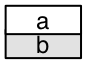
\includegraphics[scale=0.4]{e}}\tabularnewline
\hline 
\end{tabular}
\par\end{centering}

\protect\caption{\label{tab:Temporal-Relations}Temporal relations in Interval Algebra}
\end{table}


\begin{table}
\begin{centering}
\begin{tabular}{|c|c|}
\hline 
\textbf{Complement} & \textbf{Converse}\tabularnewline
\hline 
\emph{\textasciitilde{}(p) = (moFDseSdfOMP)} & \emph{!(p) = (P)}\tabularnewline
\hline 
\emph{\textasciitilde{}(pmoFD) = (seSdfOMP)} & \emph{!(pmoFD) = (dfOMP)}\tabularnewline
\hline 
\multirow{2}{*}{\textasciitilde{}() = (pmoFDseSdfOMP)} & \emph{!(mM) = (mM)}\tabularnewline
\cline{2-2} 
 & \emph{!() = ()}\tabularnewline
\hline 
\textbf{Intersection} & \textbf{Union}\tabularnewline
\hline 
\emph{(pmo)\textasciicircum{}(FDseS) = ()} & \emph{(pmo)+(FDseS) = (pmoFDseS)}\tabularnewline
\hline 
\emph{(pFsSf)\textasciicircum{}(pmoFD) = (pF)} & \emph{(pFsSf)+(pmoFD) = (pmoFDsSf)}\tabularnewline
\hline 
\emph{(pmo)\textasciicircum{}(pmo) = (pmo)} & \emph{(pmo)+(pmo) = (pmo)}\tabularnewline
\hline 
\multicolumn{2}{|c|}{\textbf{Composition}}\tabularnewline
\hline 
\multicolumn{2}{|c|}{\emph{(m).(m) = (p)}}\tabularnewline
\hline 
\multicolumn{2}{|c|}{\emph{(pm).(pm) = (p)}}\tabularnewline
\hline 
\multicolumn{2}{|c|}{\emph{(oFD).(oFDseS) = (pmoFD)}}\tabularnewline
\hline 
\end{tabular}
\par\end{centering}

\protect\caption{\label{tab:Examples-of-operations}Examples of operations on relations}
\end{table}


\begin{table}
\begin{tabular}{|c|c|c|c|c|c|c|c|c|c|c|c|c|c|}
\hline 
 & \textbf{p} & \textbf{m} & \textbf{o} & \textbf{F} & \textbf{D} & \textbf{s} & \textbf{e} & \textbf{S} & \textbf{d} & \textbf{f} & \textbf{O} & \textbf{M} & \textbf{P}\tabularnewline
\hline 
\textbf{p} & \emph{(p)} & \emph{(p)} & \emph{(p)} & \emph{(p)} & \emph{(p)} & \emph{(p)} & \emph{(p)} & \emph{(p)} & \emph{(pmosd)} & \emph{(pmosd)} & \emph{(pmosd)} & \emph{(pmosd)} & \emph{full}\tabularnewline
\hline 
\textbf{m} & \emph{(p)} & \emph{(p)} & \emph{(p)} & \emph{(p)} & \emph{(p)} & \emph{(m)} & \emph{(m)} & \emph{(m)} & \emph{(osd)} & \emph{(osd)} & \emph{(osd)} & \emph{(Fef)} & \emph{(DSOMP)}\tabularnewline
\hline 
\textbf{o} & \emph{(p)} & \emph{(p)} & \emph{(pmo)} & \emph{(pmo)} & \emph{(pmoFD)} & \emph{(o)} & \emph{(o)} & \emph{(oFD)} & \emph{(osd)} & \emph{(osd)} & \emph{concur} & \emph{(DSO)} & \emph{(DSOMP)}\tabularnewline
\hline 
\textbf{F} & \emph{(p)} & \emph{(m)} & \emph{(o)} & \emph{(F)} & \emph{(D)} & \emph{(o)} & \emph{(F)} & \emph{(D)} & \emph{(osd)} & \emph{(Fef)} & \emph{(DSO)} & \emph{(DSO)} & \emph{(DSOMP)}\tabularnewline
\hline 
\textbf{D} & \emph{(pmoFD)} & \emph{(oFD)} & \emph{(oFD)} & \emph{(D)} & \emph{(D)} & \emph{(oFD)} & \emph{(D)} & \emph{(D)} & \emph{concur} & \emph{(DSO)} & \emph{(DSO)} & \emph{(DSO)} & \emph{(DSOMP)}\tabularnewline
\hline 
\textbf{s} & \emph{(p)} & \emph{(p)} & \emph{(pmo)} & \emph{(pmo)} & \emph{(pmoFD)} & \emph{(s)} & \emph{(s)} & \emph{(seS)} & \emph{(d)} & \emph{(d)} & \emph{(dfO)} & \emph{(M)} & \emph{(P)}\tabularnewline
\hline 
\textbf{e} & \emph{(p)} & \emph{(m)} & \emph{(o)} & \emph{(F)} & \emph{(D)} & \emph{(s)} & \emph{(e)} & \emph{(S)} & \emph{(d)} & \emph{(f)} & \emph{(O)} & \emph{(M)} & \emph{(P)}\tabularnewline
\hline 
\textbf{S} & \emph{(pmoFD)} & \emph{(oFD)} & \emph{(oFD)} & \emph{(D)} & \emph{(D)} & \emph{(seS)} & \emph{(S)} & \emph{(S)} & \emph{(dfO)} & \emph{(O)} & \emph{(O)} & \emph{(M)} & \emph{(P)}\tabularnewline
\hline 
\textbf{d} & \emph{(p)} & \emph{(p)} & \emph{(pmosd)} & \emph{(pmosd)} & \emph{full} & \emph{(d)} & \emph{(d)} & \emph{(dfOMP)} & \emph{(d)} & \emph{(d)} & \emph{(dfOMP)} & \emph{(P)} & \emph{(P)}\tabularnewline
\hline 
\textbf{f} & \emph{(p)} & \emph{(m)} & \emph{(osd)} & \emph{(Fef)} & \emph{(DSOMP)} & \emph{(d)} & \emph{(f)} & \emph{(OMP)} & \emph{(d)} & \emph{(f)} & \emph{(OMP)} & \emph{(P)} & \emph{(P)}\tabularnewline
\hline 
\textbf{O} & \emph{(pmoFD)} & \emph{(oFD)} & \emph{concur} & \emph{(DSO)} & \emph{(DSOMP)} & \emph{(dfO)} & \emph{(O)} & \emph{(OMP)} & \emph{(dfO)} & \emph{(O)} & \emph{(OMP)} & \emph{(P)} & \emph{(P)}\tabularnewline
\hline 
\textbf{M} & \emph{(pmoFD)} & \emph{(seS)} & \emph{(dfO)} & \emph{(M)} & \emph{(P)} & \emph{(dfO)} & \emph{(M)} & \emph{(P)} & \emph{(dfO)} & \emph{(M)} & \emph{(P)} & \emph{(P)} & \emph{(P)}\tabularnewline
\hline 
\textbf{P} & \emph{full} & \emph{(dfOMP)} & \emph{(dfOMP)} & \emph{(P)} & \emph{(P)} & \emph{(dfOMP)} & \emph{(P)} & \emph{(P)} & \emph{(dfOMP)} & \emph{(P)} & \emph{(P)} & \emph{(P)} & \emph{(P)}\tabularnewline
\hline 
\end{tabular}

\protect\caption{\label{tab:Composition}Composition in Interval Algebra}
\end{table}



\subsection{Fuzzy Interval Algebra}

The original IA provides sufficient means for crisp reasoning. Moreover,
one can use the classic IA for systems that have their knowledge represented
as \emph{TRUE} and \emph{FALSE} propositions. However, most modern
inference engines utilise some sort of fuzzy/probabilistic representation
instead of (or in parallel to) the old-fashioned binary ones. Therefore,
such systems will not be able to use IA in it's basic form. Accordingly,
a substantial amount of work has been carried out to adapt IA to the
aforementioned paradigms. Related works that have been done in this
regards fall into two general categories: I) Probabilistic extensions
and II) Fuzzy models of IA. Each of these approaches are designed
to solve a different set of problems/setups.

Probabilistic models are usually adopted in scenarios where there
is some level of uncertainty involved in reasoning about given pieces
of knowledge. The probabilistic methods themselves are scattered in
many different sub-paradigms. So in order to offer a generalised solution
that could be adopted by all systems in which some probabilistic representations
is used, it is often the case that probabilistic extensions of IA
expand on the concept of \textquotedbl{}probability distributions\textquotedbl{}.

Keyvan should briefly explain why we didn't just use their work


\section{A Trapezium Model of Fuzzy Intervals}

Keyvan will explain the modeling of events as trapeziums with beginning,
middle and end, including a pretty diagram of a trapezium


\section{Defining Fuzzy Interval Relations via Convolution}

Keyvan will describe the convolution approach to fuzzy interval relations,
preferably using a diagram illustrating one example (could be transitivity
of \textquotedbl{}precedes\textquotedbl{})


\section{Probabilistic Estimation of a Fuzzy Interval Relation Composition
Table}

Keyvan will explain the approach to generating a composition table
probabilistically

A graph illustrating the transitivity of precedence rule should be
presented, because 3D graphs are pretty and shiny

We can give example results on the precedence rule, and leave full
discussion of the composition table till later..

\bibliography{allen}
 \bibliographystyle{plain}

% that's all folks

\end{document}
